\documentclass[10pt,a4paper]{article}

\usepackage[hidelinks]{hyperref}
\usepackage{amsmath}
\usepackage[margin=1.5in]{geometry}
\usepackage{graphicx}
\usepackage{caption}

\begin{document}
\twocolumn


\section{Decentralised Navigation}
This section of the project was developed by Paul Durbaba (pd452). Trading of coverage regions was used to ensure that robots have different regions to cover, and a combination of the spanning tree approach with some extra navigation and collision avoidance was used for navigation of these regions.

\subsection{Region Trading}
The region trader works by using an auction of grid cells available. When two robots are within range of each other, they start a trade, with all cells previously owned by either for sale. All robots start out believing that they own the entire world. Robots first purchase the position they are currently at (the trade is aborted if one of the robots is outside of the for sale region), and then expand outwards from this using breadth first search.

To avoid a robot getting trapped in a corner, a robot is able to purchase cells already purchased by the other robot should it run out of cells to buy, which introduces two complications: First, it is possible that buying a cell owned by the other robot would split that robot's region in two. Second, it is now possible for one robot to buy the position of the other, and hence the other robot ends up outside it's own region.

To deal with the first, I example the 3x3 grid around the other robot's previously owned cell, to ensure that all cells owned by that robot in this 3x3 are connected. The second problem is dealt with by making robots navigate using RRT back to their region if they find themselves outside it.

This region trading algorithm converges (meaning that no robots have intersecting regions) in about 10 random trades with 3 robots. In general, the algorithm would require every robot to meet with every other robot to guarantee convergence, thus taking $O(n^2)$ random trials, which I verified using a script to count the number of trials required for different numbers of robots. However, in practice this is not so much of a problem because robots trade regions with nearby robots, which are the robots that would otherwise have overlapping regions.

\subsection{Navigation}
Robots use the MST approach to navigate within their own regions, resorting to RRT should they find themselves outside their region. There is a two phase collision avoidance system used to prevent collisions both with the world and with other robots, that operates using LIDAR and range/bearing measurements only.

In the first phase of collision avoidance, robots slow down and change their bearing slightly to avoid colliding with the obstacle. This uses the front left / front right LIDAR sensors for the world, and with other robots, the bearing is adjusted to rotate away from the imaginary line that would connect the two robots.

The second phase, when the current path is certain to result in a collision, is to drop the current path and revert to rule based navigation until the robot has rotated sufficiently that they would no longer collide if they moved forward. This can then result in the robot navigating outside it's region and having to use RRT to re-enter it.

\begin{figure}
	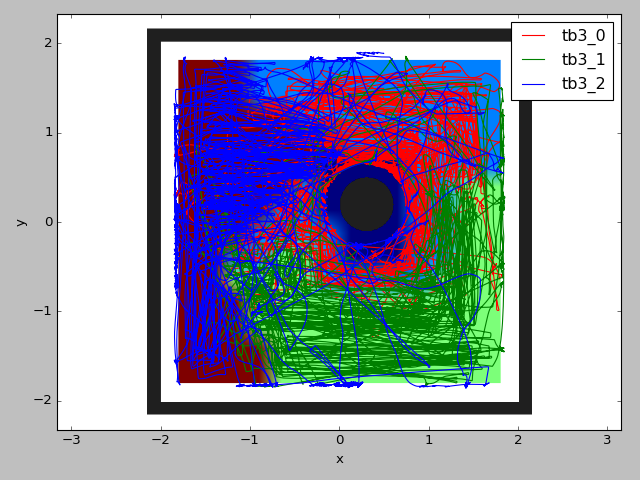
\includegraphics[width=\columnwidth]{dec_t2_cover.png}
	\caption{Robot trajectories within regions after 8000 seconds}
    \label{fig:decCover}
\end{figure}




Figure \ref{fig:decCover} shows the resulting trajectories of the robots within their regions, based on outputting each robot's position 10 times per second. By counting how often they fall inside their regions, robots 0 (red line on blue) ,1 (green on green) and 2 (blue line on brown) spend 84\%, 91\% and 70\% of their time within their own regions respectively.

\begin{figure}
	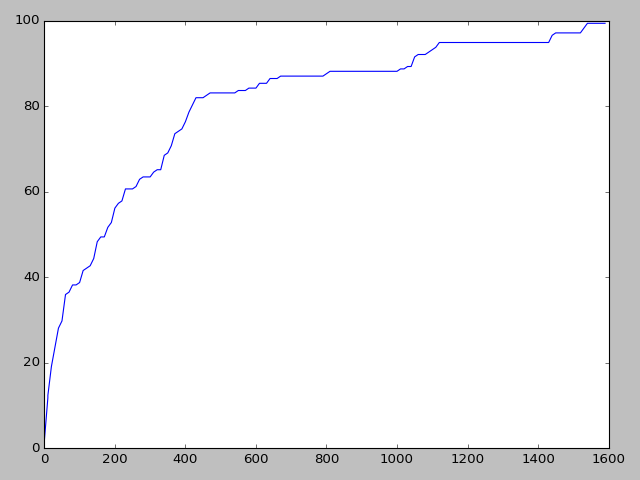
\includegraphics[width=\columnwidth]{dec_t2_line_percent.png}
	\caption{Coverage (percent of region cells out of 178) / Time (seconds)}
    \label{fig:decLine}
\end{figure}

Figure \ref{fig:decLine} shows the number of grid cells covered over time, showing that after 500 seconds the robots are able to cover 80\% of the world. The robots are programmed to move very slowly (0.15 m/s), but even at that speed localization errors will result in some cells being missed on some laps of the MST. However, after 1600 seconds each of the grid cells is able to be covered.


\section{Evaluation}
\section{Conclusions}

\end{document}